\documentclass[tikz,border=10pt]{standalone}
\usepackage{amsmath,amssymb}
\usetikzlibrary{matrix,positioning,backgrounds,fit,calc}

\begin{document}
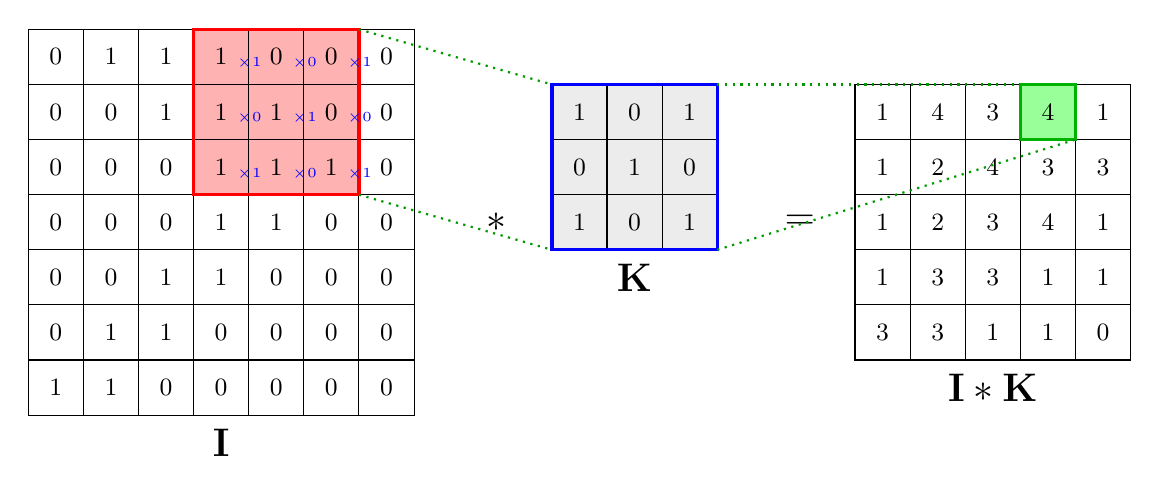
\begin{tikzpicture}[
    cell/.style={minimum size=7mm, draw, outer sep=0pt, inner sep=0pt, font=\small},
    redhighlight/.style={fill=red!30},
    greenhighlight/.style={fill=green!40},
    kernelcell/.style={minimum size=7mm, draw, outer sep=0pt, inner sep=0pt, fill=gray!15, font=\small},
]

% Cell size
\pgfmathsetmacro{\cs}{0.7}

% === Input Matrix I (7x7) ===
% Data matches the original image
% Row 0: 0,1,1,1,0,0,0
\node[cell] at (0*\cs, 0) {0};
\node[cell] at (1*\cs, 0) {1};
\node[cell] at (2*\cs, 0) {1};
\node[cell, redhighlight] at (3*\cs, 0) {1};
\node[cell, redhighlight] at (4*\cs, 0) {0};
\node[cell, redhighlight] at (5*\cs, 0) {0};
\node[cell] at (6*\cs, 0) {0};

% Row 1: 0,0,1,1,1,0,0
\node[cell] at (0*\cs, -1*\cs) {0};
\node[cell] at (1*\cs, -1*\cs) {0};
\node[cell] at (2*\cs, -1*\cs) {1};
\node[cell, redhighlight] at (3*\cs, -1*\cs) {1};
\node[cell, redhighlight] at (4*\cs, -1*\cs) {1};
\node[cell, redhighlight] at (5*\cs, -1*\cs) {0};
\node[cell] at (6*\cs, -1*\cs) {0};

% Row 2: 0,0,0,1,1,1,0
\node[cell] at (0*\cs, -2*\cs) {0};
\node[cell] at (1*\cs, -2*\cs) {0};
\node[cell] at (2*\cs, -2*\cs) {0};
\node[cell, redhighlight] at (3*\cs, -2*\cs) {1};
\node[cell, redhighlight] at (4*\cs, -2*\cs) {1};
\node[cell, redhighlight] at (5*\cs, -2*\cs) {1};
\node[cell] at (6*\cs, -2*\cs) {0};

% Row 3: 0,0,0,1,1,0,0
\node[cell] at (0*\cs, -3*\cs) {0};
\node[cell] at (1*\cs, -3*\cs) {0};
\node[cell] at (2*\cs, -3*\cs) {0};
\node[cell] at (3*\cs, -3*\cs) {1};
\node[cell] at (4*\cs, -3*\cs) {1};
\node[cell] at (5*\cs, -3*\cs) {0};
\node[cell] at (6*\cs, -3*\cs) {0};

% Row 4: 0,0,1,1,0,0,0
\node[cell] at (0*\cs, -4*\cs) {0};
\node[cell] at (1*\cs, -4*\cs) {0};
\node[cell] at (2*\cs, -4*\cs) {1};
\node[cell] at (3*\cs, -4*\cs) {1};
\node[cell] at (4*\cs, -4*\cs) {0};
\node[cell] at (5*\cs, -4*\cs) {0};
\node[cell] at (6*\cs, -4*\cs) {0};

% Row 5: 0,1,1,0,0,0,0
\node[cell] at (0*\cs, -5*\cs) {0};
\node[cell] at (1*\cs, -5*\cs) {1};
\node[cell] at (2*\cs, -5*\cs) {1};
\node[cell] at (3*\cs, -5*\cs) {0};
\node[cell] at (4*\cs, -5*\cs) {0};
\node[cell] at (5*\cs, -5*\cs) {0};
\node[cell] at (6*\cs, -5*\cs) {0};

% Row 6: 1,1,0,0,0,0,0
\node[cell] at (0*\cs, -6*\cs) {1};
\node[cell] at (1*\cs, -6*\cs) {1};
\node[cell] at (2*\cs, -6*\cs) {0};
\node[cell] at (3*\cs, -6*\cs) {0};
\node[cell] at (4*\cs, -6*\cs) {0};
\node[cell] at (5*\cs, -6*\cs) {0};
\node[cell] at (6*\cs, -6*\cs) {0};

% Red border around 3x3 region (cols 3-5, rows 0-2)
\draw[red, very thick] (3*\cs-0.35, 0.35) rectangle (5*\cs+0.35, -2*\cs-0.35);

% Small subscript annotations in red region (kernel weights) - positioned at lower right
\node[font=\tiny, blue, anchor=south west] at (3*\cs+0.08, -0.28) {$\times 1$};
\node[font=\tiny, blue, anchor=south west] at (4*\cs+0.08, -0.28) {$\times 0$};
\node[font=\tiny, blue, anchor=south west] at (5*\cs+0.08, -0.28) {$\times 1$};
\node[font=\tiny, blue, anchor=south west] at (3*\cs+0.08, -1*\cs-0.28) {$\times 0$};
\node[font=\tiny, blue, anchor=south west] at (4*\cs+0.08, -1*\cs-0.28) {$\times 1$};
\node[font=\tiny, blue, anchor=south west] at (5*\cs+0.08, -1*\cs-0.28) {$\times 0$};
\node[font=\tiny, blue, anchor=south west] at (3*\cs+0.08, -2*\cs-0.28) {$\times 1$};
\node[font=\tiny, blue, anchor=south west] at (4*\cs+0.08, -2*\cs-0.28) {$\times 0$};
\node[font=\tiny, blue, anchor=south west] at (5*\cs+0.08, -2*\cs-0.28) {$\times 1$};

% Label for I
\node at (3*\cs, -6*\cs-0.7) {\Large $\mathbf{I}$};

% === Convolution operator ===
\pgfmathsetmacro{\convx}{8*\cs}
\node at (\convx, -3*\cs) {\Large $*$};

% === Kernel K (3x3) - vertically centered ===
\pgfmathsetmacro{\kx}{9.5*\cs}
\pgfmathsetmacro{\ky}{-2*\cs}  % Center kernel vertically around middle of input

\node[kernelcell] at (\kx+0*\cs, \ky+1*\cs) {1};
\node[kernelcell] at (\kx+1*\cs, \ky+1*\cs) {0};
\node[kernelcell] at (\kx+2*\cs, \ky+1*\cs) {1};
\node[kernelcell] at (\kx+0*\cs, \ky+0*\cs) {0};
\node[kernelcell] at (\kx+1*\cs, \ky+0*\cs) {1};
\node[kernelcell] at (\kx+2*\cs, \ky+0*\cs) {0};
\node[kernelcell] at (\kx+0*\cs, \ky-1*\cs) {1};
\node[kernelcell] at (\kx+1*\cs, \ky-1*\cs) {0};
\node[kernelcell] at (\kx+2*\cs, \ky-1*\cs) {1};

% Blue border around kernel
\draw[blue, very thick] (\kx-0.35, \ky+1*\cs+0.35) rectangle (\kx+2*\cs+0.35, \ky-1*\cs-0.35);

% Label for K
\node at (\kx+1*\cs, \ky-1*\cs-0.7) {\Large $\mathbf{K}$};

% === Equals sign ===
\pgfmathsetmacro{\eqx}{13.5*\cs}
\node at (\eqx, -3*\cs) {\Large $=$};

% === Output Matrix I*K (5x5) ===
\pgfmathsetmacro{\ox}{15*\cs}

% Row 0
\node[cell] at (\ox+0*\cs, -1*\cs) {1};
\node[cell] at (\ox+1*\cs, -1*\cs) {4};
\node[cell] at (\ox+2*\cs, -1*\cs) {3};
\node[cell, greenhighlight] at (\ox+3*\cs, -1*\cs) {4};
\node[cell] at (\ox+4*\cs, -1*\cs) {1};

% Row 1
\node[cell] at (\ox+0*\cs, -2*\cs) {1};
\node[cell] at (\ox+1*\cs, -2*\cs) {2};
\node[cell] at (\ox+2*\cs, -2*\cs) {4};
\node[cell] at (\ox+3*\cs, -2*\cs) {3};
\node[cell] at (\ox+4*\cs, -2*\cs) {3};

% Row 2
\node[cell] at (\ox+0*\cs, -3*\cs) {1};
\node[cell] at (\ox+1*\cs, -3*\cs) {2};
\node[cell] at (\ox+2*\cs, -3*\cs) {3};
\node[cell] at (\ox+3*\cs, -3*\cs) {4};
\node[cell] at (\ox+4*\cs, -3*\cs) {1};

% Row 3
\node[cell] at (\ox+0*\cs, -4*\cs) {1};
\node[cell] at (\ox+1*\cs, -4*\cs) {3};
\node[cell] at (\ox+2*\cs, -4*\cs) {3};
\node[cell] at (\ox+3*\cs, -4*\cs) {1};
\node[cell] at (\ox+4*\cs, -4*\cs) {1};

% Row 4
\node[cell] at (\ox+0*\cs, -5*\cs) {3};
\node[cell] at (\ox+1*\cs, -5*\cs) {3};
\node[cell] at (\ox+2*\cs, -5*\cs) {1};
\node[cell] at (\ox+3*\cs, -5*\cs) {1};
\node[cell] at (\ox+4*\cs, -5*\cs) {0};

% Green border around highlighted cell
\draw[green!70!black, very thick] (\ox+3*\cs-0.35, -1*\cs+0.35) rectangle (\ox+3*\cs+0.35, -1*\cs-0.35);

% Label for I*K
\node at (\ox+2*\cs, -5*\cs-0.7) {\Large $\mathbf{I} * \mathbf{K}$};

% === Dotted lines connecting regions ===
% From red region corners to kernel
\draw[dotted, thick, green!60!black] (5*\cs+0.35, 0.35) -- (\kx-0.35, \ky+1*\cs+0.35);
\draw[dotted, thick, green!60!black] (5*\cs+0.35, -2*\cs-0.35) -- (\kx-0.35, \ky-1*\cs-0.35);

% From kernel corners to output cell
\draw[dotted, thick, green!60!black] (\kx+2*\cs+0.35, \ky+1*\cs+0.35) -- (\ox+3*\cs-0.35, -1*\cs+0.35);
\draw[dotted, thick, green!60!black] (\kx+2*\cs+0.35, \ky-1*\cs-0.35) -- (\ox+3*\cs+0.35, -1*\cs-0.35);

\end{tikzpicture}
\end{document}
